\documentclass[12pt]{article}

\usepackage[margin=22mm]{geometry}
\usepackage[labelfont=bf,font=small]{caption}
\captionsetup{skip=4pt}
\setlength{\textfloatsep}{10pt plus 2pt minus 2pt}
\setlength{\floatsep}{8pt plus 2pt minus 2pt}
\setlength{\intextsep}{8pt plus 2pt minus 2pt}

% Figures / TikZ
\usepackage{graphicx}
\usepackage{tikz}
\usepackage{pgfplots}
\pgfplotsset{compat=1.18}
\usetikzlibrary{arrows.meta,positioning,fit}
\usepackage{subcaption}   % ← subfigure 用
\usepackage{float}        % ← [H]
\usepackage{placeins}     % ← \FloatBarrier

\pagestyle{empty}

\begin{document}

% ------------------ Title ------------------
\vspace*{-6mm}
\begin{center}
{\LARGE \textbf{Supplementary Figures and Tables for}}\\[2mm]
{\Large \textit{“FeFET CMOS 0.18~$\mu$m Integration Study”}}
\end{center}
\vspace{2mm}

% ================== Page 1 ==================
% Fig.1
\begin{figure}[H]
\centering
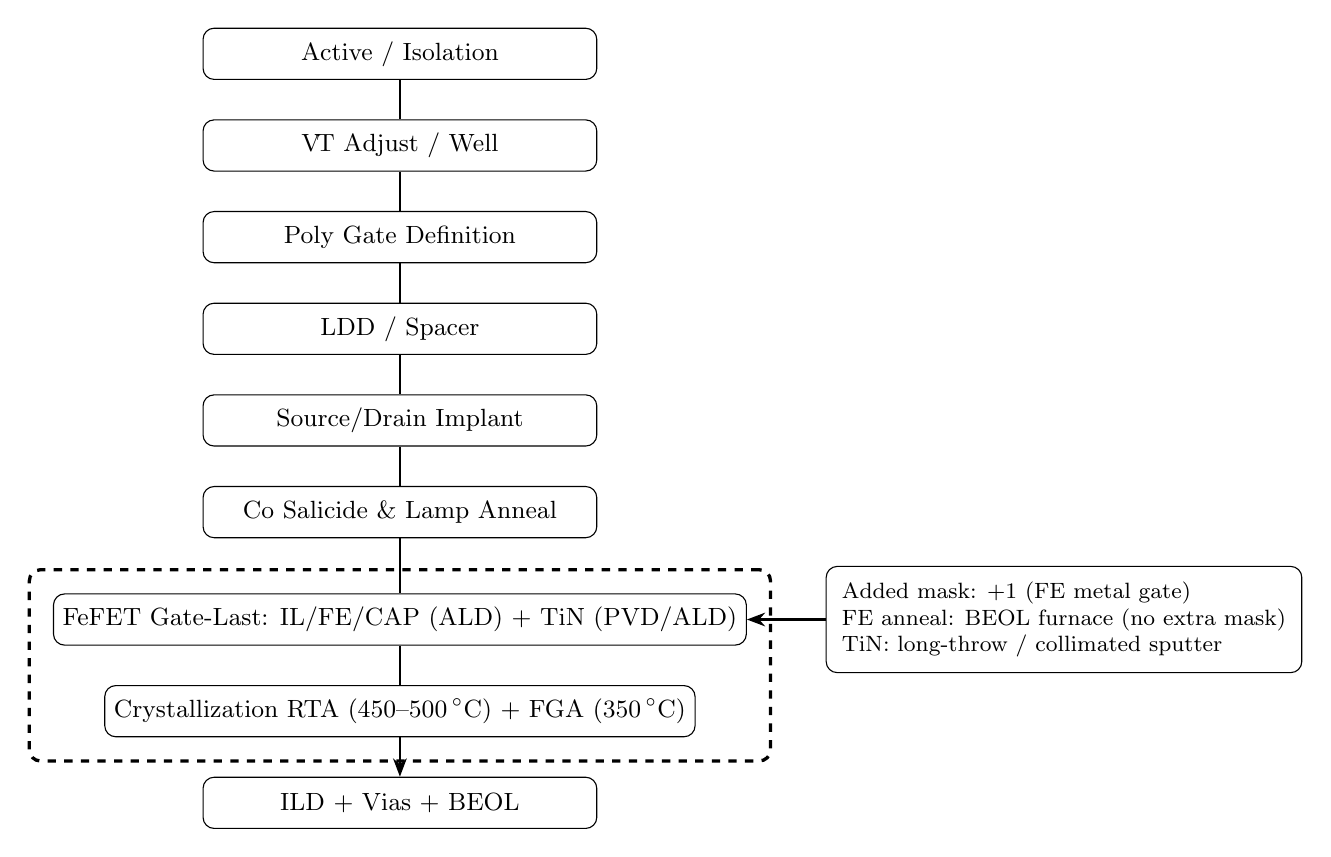
\begin{tikzpicture}[
  node distance=5mm,
  stage/.style={draw,rounded corners,minimum width=50mm,minimum height=6.5mm,
                align=center,font=\small},
  arr/.style={-{Stealth},thick},
  note/.style={draw,rounded corners,align=left,font=\footnotesize,inner sep=2mm}
]
\node[stage] (act)  {Active / Isolation};
\node[stage,below=of act] (vt)   {V\!T Adjust / Well};
\node[stage,below=of vt]  (poly) {Poly Gate Definition};
\node[stage,below=of poly] (ldd) {LDD / Spacer};
\node[stage,below=of ldd]  (sd)  {Source/Drain Implant};
\node[stage,below=of sd]   (sal) {Co Salicide \& Lamp Anneal};

\node[stage,below=7mm of sal]  (fegate) {FeFET Gate-Last: IL/FE/CAP (ALD) + TiN (PVD/ALD)};
\node[stage,below=of fegate]   (rta)   {Crystallization RTA (450--500\,$^{\circ}$C) + FGA (350\,$^{\circ}$C)};
\node[stage,below=of rta]      (ild)   {ILD + Vias + BEOL};

\draw[arr] (act) -- (vt) -- (poly) -- (ldd) -- (sd) -- (sal) -- (fegate) -- (rta) -- (ild);

\node[draw,dashed,rounded corners,very thick,fit=(fegate)(rta),inner sep=3mm] (box) {};
\node[note,anchor=west,right=10mm of fegate] (n1)
  {Added mask: +1 (FE metal gate)\\
   FE anneal: BEOL furnace (no extra mask)\\
   TiN: long-throw / collimated sputter};
\draw[arr] (n1.west) -- ++(-6mm,0) |- (fegate.east);
\end{tikzpicture}
\caption{Placement of the FeFET gate-last module within the 0.18~$\mu$m CMOS baseline (vertical layout).}
\label{fig:flow}
\end{figure}

\vspace{6mm}

% Table I
\begin{table}[H]
\centering
\caption{Added masks / process steps relative to baseline logic.}
\label{tab:masks}
\begin{tabular}{|c|c|p{85mm}|}
\hline
\textbf{Step} & \textbf{Mask} & \textbf{Comment}\\ \hline
FE metal gate & +1 & Reuse analog option route\\
FE anneal     & 0  & Performed in BEOL furnace (no extra mask)\\ \hline
\end{tabular}
\end{table}

% --- 強制的にページを切る ---
\FloatBarrier
\clearpage

% ================== Page 2 ==================
% Fig.2 Endurance
\begin{figure}[H]
\centering
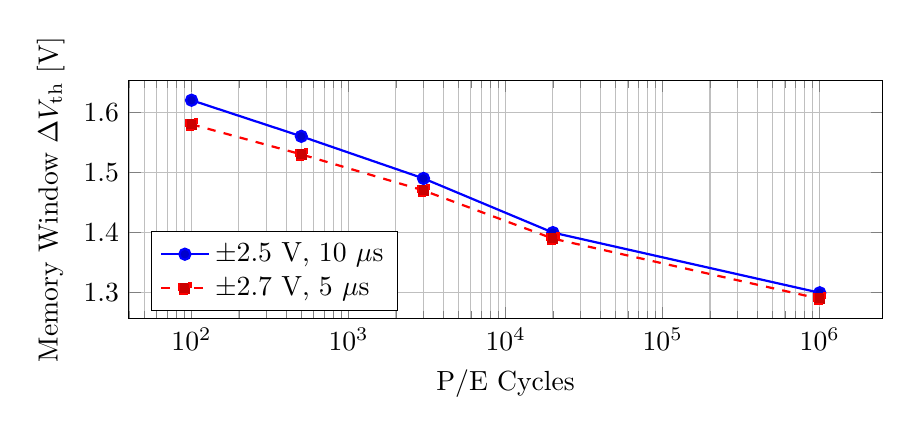
\begin{tikzpicture}
\begin{axis}[
  width=0.92\linewidth,height=0.38\linewidth,
  xlabel={P/E Cycles}, xmode=log, log basis x=10,
  ylabel={Memory Window $\Delta V_{\mathrm{th}}$ [V]},
  grid=both, legend pos=south west, legend cell align=left
]
\addplot+[mark=*,thick] coordinates {(1e2,1.62) (5e2,1.56) (3e3,1.49) (2e4,1.40) (1e6,1.30)};
\addlegendentry{$\pm 2.5$ V, 10 $\mu$s}
\addplot+[mark=square*, dashed,thick] coordinates {(1e2,1.58) (5e2,1.53) (3e3,1.47) (2e4,1.39) (1e6,1.29)};
\addlegendentry{$\pm 2.7$ V, 5 $\mu$s}
\end{axis}
\end{tikzpicture}
\caption{Schematic endurance behavior of HZO-FeFETs in a 0.18~$\mu$m flow.}
\label{fig:endurance}
\end{figure}

\vspace{2mm}

% ===== Fig.3 Wake-up & Retention(横並び・修正版) =====
\captionsetup[sub]{font=small,skip=2pt,justification=centering}

\begin{figure}[H]
  \centering
  % 左:Wake-up
  \subcaptionbox{Wake-up}[0.48\linewidth]{%
    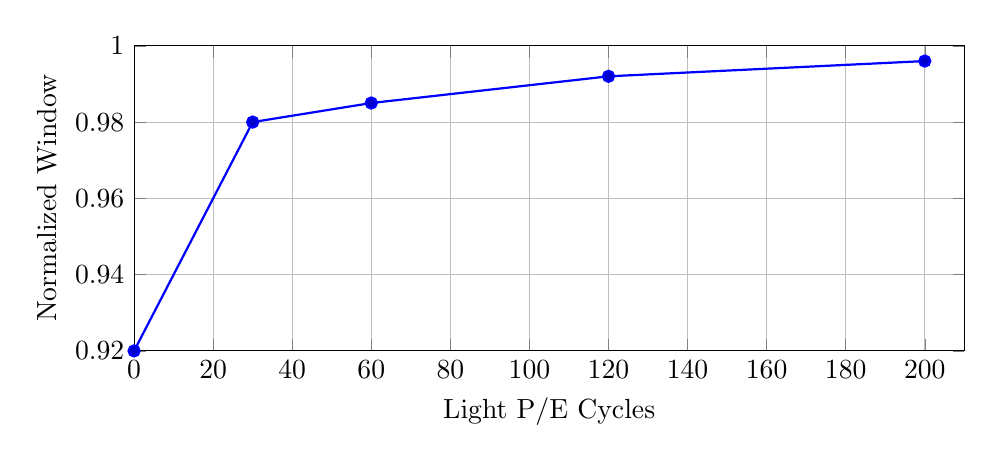
\begin{tikzpicture}
      \begin{axis}[
        width=\linewidth, height=0.45\linewidth, % ←縦幅拡大
        xmin=0, xmax=210, ymin=0.92, ymax=1.00,
        xlabel={Light P/E Cycles}, ylabel={Normalized Window},
        grid=both, tick align=inside, /pgf/number format/precision=2
      ]
        \addplot+[mark=*, thick] coordinates
          {(0,0.92) (30,0.98) (60,0.985) (120,0.992) (200,0.996)};
      \end{axis}
    \end{tikzpicture}
  }\hfill
  % 右:Retention
  \subcaptionbox{Retention at 85$^\circ$C}[0.48\linewidth]{%
    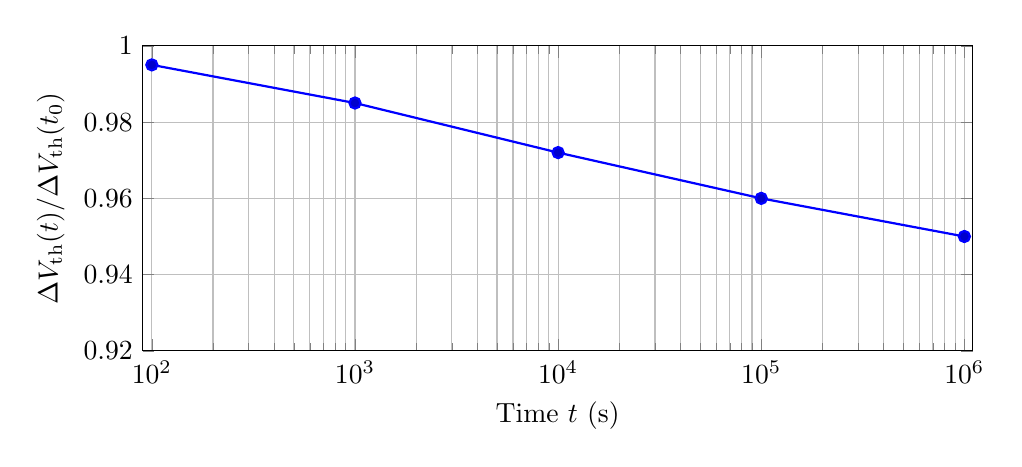
\begin{tikzpicture}
      \begin{axis}[
        width=\linewidth, height=0.45\linewidth, % ←縦幅拡大
        xmode=log, log basis x=10,
        xmin=9e1, xmax=1.1e6, ymin=0.92, ymax=1.00,
        xlabel={Time $t$ (s)}, ylabel={$\Delta V_{\mathrm{th}}(t)/\Delta V_{\mathrm{th}}(t_0)$},
        grid=both, tick align=inside
      ]
        \addplot+[mark=*, thick] coordinates
          {(1e2,0.995) (1e3,0.985) (1e4,0.972) (1e5,0.960) (1e6,0.950)};
      \end{axis}
    \end{tikzpicture}
  }
  \caption{Wake-up(左)と Retention(右)の比較。}
  \label{fig:wakeup_retention}
\end{figure}

% Fig.4 TDDB(凡例は右下)
\begin{figure}[H]
\centering
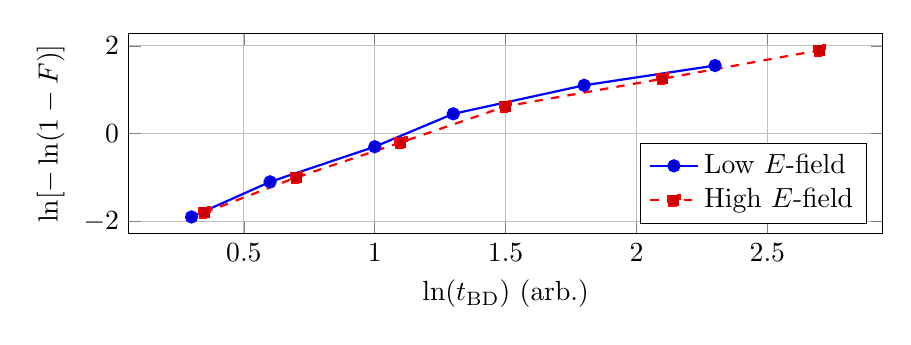
\begin{tikzpicture}
\begin{axis}[
  width=0.92\linewidth,height=0.34\linewidth,
  xlabel={$\ln(t_{\mathrm{BD}})$ (arb.)},
  ylabel={$\ln[-\ln(1-F)]$},
  grid=both, legend style={at={(0.98,0.05)},anchor=south east}, legend cell align=left
]
\addplot+[mark=*,thick] coordinates {(0.3,-1.9) (0.6,-1.1) (1.0,-0.3) (1.3,0.45) (1.8,1.10) (2.3,1.55)};
\addlegendentry{Low $E$-field}
\addplot+[mark=square*, dashed,thick] coordinates {(0.35,-1.8) (0.7,-1.0) (1.1,-0.2) (1.5,0.62) (2.1,1.25) (2.7,1.90)};
\addlegendentry{High $E$-field}
\end{axis}
\end{tikzpicture}
\caption{TDDB Weibull representation at two stress fields (illustrative).}
\label{fig:tddb}
\end{figure}

\end{document}
